\section{Exact neighborhood-subgraph extraction}
\label{sec:query}
\subsection{Task, cohorts and measurement}
The new task returns the exact induced subgraph on the vertices within $h$ hops of an input seed set $Q$. Every method must produce the same sorted vertex and undirected-edge buffers. The partition path first uses the existing boundary index to obtain candidates and then performs the exact work needed to construct the output. Two BFS controls return the same output: one uses the original graph layout and the other uses each selector's physical layout. Original vertex IDs are preserved when layouts change.

The primary workload fixes $h=1$ and $|Q|=1$, with 1,000 uniform-start and 1,000 degree-stratified-start queries per graph. Each of the eight remaining strata has 100 queries and is reported separately as context. The Stanford/Google batch completed on 8 November 2026; the in-2004/eu-2005 extension completed on 9 November using the same engine and settings. Starts exclude the earlier development, test and pilot starts. Query sets and minimum-budget configurations were fixed before timing. A common $8n$-byte mapping is added to the original minimum-budget accounting for all selectors.

\begin{table}[H]
\centering\tablefont\setlength{\tabcolsep}{5pt}
\caption{Primary workload: all partition selectors. Times are in microseconds, requested bytes in KiB ($2^{10}$ bytes). Random-P averages five seed-specific means; its P95 entry is the mean of five seed-specific P95 values, not the percentile of a pooled distribution.}
\label{tab:query-methods}
\begin{tabular}{@{}llrrrr@{}}
\toprule
Graph & Method & Memory mean & Warm-file mean & Warm-file P95 & Req. KiB \\
\midrule
Stanford & Ratio & 70.82 & 284.10 & 1215.49 & 363.33 \\
 & Ratio+ & 111.62 & 757.92 & 3627.50 & 714.01 \\
 & Degree & 87.92 & 385.92 & 2172.91 & 402.09 \\
 & CC$^2$FS & 106.63 & 739.22 & 3222.32 & 631.91 \\
 & Random-P & 92.47 & 397.26 & 1890.66 & 439.97 \\
\midrule
Google & Ratio & 3.23 & 23.22 & 63.22 & 8.99 \\
 & Ratio+ & 4.54 & 27.05 & 80.16 & 13.11 \\
 & Degree & 6.50 & 32.31 & 92.04 & 14.62 \\
 & CC$^2$FS & 7.52 & 35.54 & 103.69 & 17.29 \\
 & Random-P & 7.08 & 34.48 & 100.74 & 16.13 \\
\midrule
in-2004 & Ratio & 33.74 & 127.29 & 750.41 & 252.91 \\
 & Ratio+ & 40.91 & 160.36 & 783.84 & 336.70 \\
 & Degree & 39.97 & 153.03 & 756.46 & 282.70 \\
 & CC$^2$FS & 40.80 & 169.05 & 766.24 & 305.86 \\
 & Random-P & 38.62 & 140.27 & 690.12 & 286.14 \\
\midrule
eu-2005 & Ratio & 103.27 & 319.18 & 1326.22 & 744.72 \\
 & Ratio+ & 197.99 & 1002.93 & 6254.17 & 1763.37 \\
 & Degree & 171.45 & 692.86 & 2500.83 & 1375.68 \\
 & CC$^2$FS & 223.67 & 1224.07 & 6066.19 & 1846.35 \\
 & Random-P & 165.75 & 702.78 & 2915.45 & 1314.28 \\
\bottomrule
\end{tabular}

\end{table}

Timing starts with the native query seeds and ends after complete sorted output buffers. It includes scratch reset, candidate/frontier reads, exact processing and output construction; independent correctness checks and warmup are excluded. Each configuration has three repetitions, collapsed to a median per query before aggregation. Table~\ref{tab:query-methods} gives means over those query-level values, while P95 describes their latency distribution. Memory and warm-file measurements are kept separate.

\clearpage
\subsection{Primary comparisons and BFS controls}
In the warm-file primary workload, Ratio reduces mean complete time by $16.8$--$53.9\%$ relative to Degree and $9.3$--$54.6\%$ relative to the Random-Prune mean across the four graphs. All eight corresponding 95\% time-ratio intervals lie below one (Table~\ref{tab:query-ci}). Requested adjacency bytes also decrease in all eight comparisons. The result supports the practical value of landmark choice within the shared partition-extraction pipeline.

\begin{table}[H]
\centering\tablefont\setlength{\tabcolsep}{5pt}
\caption{Primary warm-file comparisons. Ratios are Ratio/reference, so values below one favor Ratio. Confidence intervals are paired stratified bootstrap percentile intervals with 2,000 resamples; random configurations are resampled as well as queries.}
\label{tab:query-ci}
\begin{tabular}{@{}llrcrc@{}}
\toprule
Graph & Reference & Time ratio & 95\% CI & Byte ratio & 95\% CI \\
\midrule
Stanford & Degree & 0.736 & [0.692, 0.783] & 0.904 & [0.886, 0.921] \\
Stanford & Random-P & 0.715 & [0.671, 0.758] & 0.826 & [0.798, 0.852] \\
Google & Degree & 0.719 & [0.696, 0.742] & 0.615 & [0.596, 0.635] \\
Google & Random-P & 0.673 & [0.654, 0.694] & 0.557 & [0.539, 0.576] \\
in-2004 & Degree & 0.832 & [0.779, 0.887] & 0.895 & [0.821, 0.967] \\
in-2004 & Random-P & 0.907 & [0.859, 0.955] & 0.884 & [0.837, 0.932] \\
eu-2005 & Degree & 0.461 & [0.440, 0.483] & 0.541 & [0.524, 0.558] \\
eu-2005 & Random-P & 0.454 & [0.416, 0.506] & 0.567 & [0.517, 0.618] \\
\bottomrule
\end{tabular}

\end{table}

\paragraph{Uncertainty and aggregation.}
Uniform and degree-stratified queries receive equal weight in the primary aggregate. The bootstrap resamples queries within each stratum, keeping method observations paired. The random reference additionally resamples the five seed configurations. The intervals quantify sampling variation within the evaluated graph/workload configurations. Ratios divide the mean times of the compared methods. Separate workload-specific comparisons are retained in the frozen uncertainty files; all primary point estimates against Degree and Random-Prune are below one for both start distributions.

\begin{table}[H]
\centering\tablefont\setlength{\tabcolsep}{5pt}
\caption{Primary workload BFS controls. Times are mean microseconds. Same-layout BFS uses Ratio's physical layout. The last column divides Ratio partition time by same-layout BFS time.}
\label{tab:bfs}
\begin{tabular}{@{}llrrrr@{}}
\toprule
Graph & Mode & Ratio partition & Original BFS & Same-layout BFS & Ratio/same \\
\midrule
Stanford & Memory & 70.82 & 32.05 & 31.36 & 2.26 \\
Stanford & Warm file & 284.10 & 114.16 & 83.00 & 3.42 \\
Google & Memory & 3.23 & 2.34 & 2.33 & 1.38 \\
Google & Warm file & 23.22 & 42.95 & 29.57 & 0.79 \\
in-2004 & Memory & 33.74 & 23.47 & 23.44 & 1.44 \\
in-2004 & Warm file & 127.29 & 49.89 & 56.70 & 2.24 \\
eu-2005 & Memory & 103.27 & 78.46 & 78.62 & 1.31 \\
eu-2005 & Warm file & 319.18 & 158.05 & 178.64 & 1.79 \\
\bottomrule
\end{tabular}

\end{table}

Google's warm-file Ratio partition path is faster than both BFS controls. For Stanford, in-2004 and eu-2005, BFS remains faster; in memory, BFS is faster on all four graphs. The results compare landmark selection within the partition pipeline alongside direct traversal.

\clearpage
\subsection{Secondary workloads and cache scope}
Figure~\ref{fig:context} retains all eight secondary query strata on each graph. Each cell uses 100 newly generated queries. Warm-file mean time decreases in 24 of the 64 graph--reference--stratum comparisons. The figure reports each secondary stratum separately to show how performance varies with query size, radius and start distribution.

\begin{figure}[H]
\centering
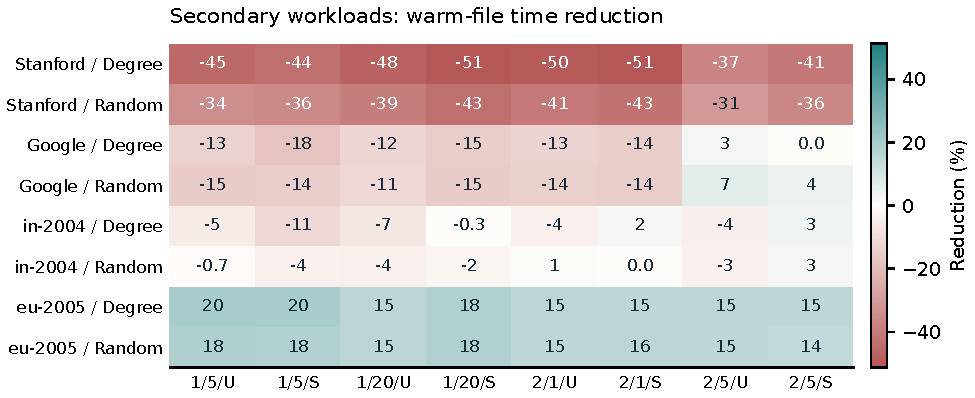
\includegraphics[width=\linewidth]{query_context.pdf}
\caption{Secondary strata: $100(1-T_{\mathrm{Ratio}}/T_{\mathrm{reference}})$ for complete warm-file query time. Labels are $h/|Q|/$start distribution, with U uniform and S degree-stratified. Positive values favor Ratio; negative values indicate additional time. Random denotes the five-seed mean.}
\label{fig:context}
\end{figure}

\paragraph{Reading volume and cache state.}
The shared reader deduplicates adjacency rows, coalesces contiguous reads and reuses rows within a query. Files are prewarmed before each process, with the same per-query warmup rule for every method. Requested bytes count unique adjacency-row requests, including frontier reads. Timed batches use warm files and recorded zero physical read bytes. Both formal batches pass exact-vertex, exact-edge, logical-reading and record-hash checks for all partition and BFS methods; validation is outside timing.
